% Template for PLoS
% Version 1.0 January 2009
%
% To compile to pdf, run:
% latex plos.template
% bibtex plos.template
% latex plos.template
% latex plos.template
% dvipdf plos.template

\documentclass[10pt]{article}

% amsmath package, useful for mathematical formulas
\usepackage{amsmath}
% amssymb package, useful for mathematical symbols
\usepackage{amssymb}

% graphicx package, useful for including eps and pdf graphics
% include graphics with the command \includegraphics
\usepackage{graphicx}

% cite package, to clean up citations in the main text. Do not remove.
\usepackage{cite}

\usepackage{color} 

% Use doublespacing - comment out for single spacing
%\usepackage{setspace} 
%\doublespacing


% Text layout
\topmargin 0.0cm
\oddsidemargin 0.5cm
\evensidemargin 0.5cm
\textwidth 16cm 
\textheight 21cm

% Bold the 'Figure #' in the caption and separate it with a period
% Captions will be left justified
\usepackage[labelfont=bf,labelsep=period,justification=raggedright]{caption}

% Use the PLoS provided bibtex style
\bibliographystyle{plos2009}

% Remove brackets from numbering in List of References
\makeatletter
\renewcommand{\@biblabel}[1]{\quad#1.}
\makeatother


% Leave date blank
\date{}

\pagestyle{myheadings}
%% ** EDIT HERE **


%% ** EDIT HERE **
%% PLEASE INCLUDE ALL MACROS BELOW

%% END MACROS SECTION

\begin{document}

% Title must be 150 characters or less
\begin{flushleft}
{\Large
\textbf{Python as a Federation Tool for GENESIS 3.0}
}
% Insert Author names, affiliations and corresponding author email.
\\
Cornelis H.$^{1,\ast}$, 
Rodriguez A. L.$^{2}$, 
Joe J. L.$^{3}$
Coop A. D.$^{4}$,
Bower J. M.$^{5}$.
\\
\bf{1} Cornelis H. Research Imaging Institute, University of Texas Health Science Center at San Antonio, San Antonio, TX, United States
\\
\bf{2} Rodriguez A. L. Research Imaging Institute, University of Texas Health Science Center at San Antonio, San Antonio, TX, United States
\\
\bf{3} Joe J. L. College of Medicine, Wonkwang University, Republic of Korea
\\
\bf{4} Coop A. D. Deptartment of Epidemiology and Biostatistics, University of Texas Health Science Center at San Antonio, San Antonio, TX, United States
\\
\bf{5} Bower J. M. Research Imaging Institute, University of Texas Health Science Center at San Antonio, San Antonio, TX, United States
\\
$\ast$ E-mail: Corresponding Hugo.Cornelis@gmail.com
\end{flushleft}

% Please keep the abstract between 250 and 300 words
\section*{Abstract}
Python is a script programing language that provides a rich set of freely available open source libraries.
% Citation removed from abstract \,\cite{langtangen04:python-scrip-comput-scien}.
With a clean dynamic object-oriented design producing highly readable code,
it is widely employed in specialized areas of systems
integration.
% Citation removed from abstract (e.g\,.~\cite{thiruvathukal01:web-progr-python}).

An important feature of the latest version of the GENESIS neural simulation platform, GENESIS 3.0, is that it is composed of self-contained software components that conform to the Computational Biology Initiative federated software architecture.
% Citation removed from abstract \,\cite{cornelis08:cbi-archit-comput-simul-realis}.  
This modular software architecture allows separate Python bindings to be defined for the different software components that support simulator functionality.

Currently, there are many available technologies that could simplify the binding of Python libraries to GENESIS 3.0.  We employ a simplified wrapper and interface
generator that
% Citation removed from abstract \,\cite{08:simpl-wrapp-inter-gener}).  
examines an application programming interface and makes it available to a scripting language.
However, additional code is required as neither a low-level application programming interface nor an application programming interface
generated by the simplified wrapper and interface
generator possess the high-level functionality necessary to
complete the binding of software components in a federated software architecture.
% Citation removed from abstract \,\cite{08:swig-python}. 
We employ self-query and dynamic
compilation techniques to minimize the maintenance costs of existing
code and simplify the addition of new components designed to extend simulator functionality.

Our approach is illustrated with two examples: (1) a Python script that
generates, runs, and displays the output of a simple single-compartment model neuron, and (2) the application of Python bindings
to connect the GENESIS 3.0 simulator to Blender, an open source 3D content
creation suite.  % We use these bindings to visualize 3D models based on
% electron microscopy and convert them to computational models.
% Citation removed from abstract \,\cite{cornelis08:model-neuros-genes}.

% Please keep the Author Summary between 150 and 200 words
% Use first person. PLoS ONE authors please skip this step. 
% Author Summary not valid for PLoS ONE submissions.   
% \section*{Author Summary}

\section*{Introduction}
Historically, there have been fundamental differences between system 
programming languages such as C or C++ and
scripting languages such as the Unix shells,
Perl\,\cite{wall99:perl-progr-refer-guide},
Python\,\cite{martelli06:python-nutsh},
Rexx\,\cite{o'hara88:moder-progr-using-rexx},
Tcl\,\cite{ousterhout94:tcl-tk-toolk}, or Visual Basic.  System programming languages start from the most primitive computer elements, the words of memory. They usually
require pre-declared data types and are designed to manage the complexity of
building data structures and algorithms from scratch.  Alternatively, as a replacement for shell scripts, scripting languages assume the existence of a set of software components and are designed to assemble or `glue' these components together. The fact that
they typically require neither pre-declared data types nor a
visible compilation step simplifies the integration of pre-existing software components and allows for rapid software development.  They are also often small or `lightweight' languages, thus suited to being embedded in pre-existing software, operate in an interpreted development environment, and provide a higher level of programming than a system language in the sense that on average a single statement in a scripting language does more
work. For example, a typical statement in a system programming
language executes about five machine instructions, whereas in a
scripting language a typical statement may execute hundreds or thousands of machine instructions\,\cite{ousterhout98:scrip}.

%9.  L. Wall, T. Christiansen, and R. Schwartz, Programming Perl, Second Edition, O'Reilly and Associates, ISBN 1-56592-149-6, 1996.
%4. M. Lutz, Programming Python, O'Reilly, ISBN 1-56592-197-6, 1996.
%6. R. O'Hara and D. Gomberg, Modern Programming Using REXX, Prentice Hall, ISBN 0-13-597329-5, 1988.
%8.  J. Ousterhout, Tcl and the Tk Toolkit, Addison-Wesley, ISBN 0-201-63337-X, 1994.
% 1. John K. Ousterhout (1998) Scripting: Higher Level Programming for the 21st Century. IEEE COMPUTER 31: 23-30.

A scripting language is not a replacement for a system programming language, or vice versa, as each is suited to a different set of tasks. System programming languages typically require large amounts of `boilerplate' and conversion code to connect software components together, a functionality that is implicit in scripting languages. When execution speed is critical, a system programming language can often run several orders of magnitude faster than a scripting language due to a reduced requirement for run-time checks.

The strongly typed nature of system programming languages discourages
reuse. Scripting languages, on the other hand, have actually
stimulated significant software reuse. They use a model where
interesting components are built in a system programming language and
then glued together into applications.
This division of labor provides a natural framework for reusability.
When well-defined interfaces between components and scripts exist, software reuse becomes easy.
In this sense scripting and system programming are symbiotic. Used together, they produce programming environments of exceptional power where applications can be developed
five to ten times more rapidly than when a system programming language is used.
%: system programming languages are used to create functional components
% which are then be assembled using scripting languages.

In summary, system programming languages are well suited for building functional
components where there is a requirement for computing speed because data structures and
algorithms are complex, whereas, scripting languages are well suited for assembling
applications when complexity is in the connections. With an
increasing requirement for software integration, scripting is
providing an important programming paradigm.

Here, we illustrate the use of the general purpose Python scripting
language for making high performance simulation software coded in
system programming languages accessible to neuroscientists and
biologists.

% Results and Discussion can be combined.
\section*{Results}

PyGENESIS was a version of the GEneral NEural SImulation System (GENESIS) developed by Michael Vanier in the late 1990's. It replaced the standard GENESIS Script Language Interface (SLI) with a
Python interface. This Python-enabled version of GENESIS was never
publicly released.  However, with the increased sophistication of the Python
platform and development of G-3 in compliance with the Computational Biology Initiative (CBI) federated software architecture (referred to as the CBI architecture), Python interfaces have been developed for several of the core
simulator components.  While it is possible to drive each
component in isolation from these interfaces, in the following sections, we
show how individual components may be integrated via Python interfaces to create a simple simulator.

\subsection*{A Python Enabled Neural Simulator}

Python uses modules to group related functions together.  The Python
bindings of the G-3 simulator use modules to separate interfaces for
simple models with many default settings (e.g. to start a new research
project) from more complicated interfaces that expose the full
functionality of the simulator.

As an example the {\tt Neurospaces.SingleCellContainer} module
contains functions to simplify simulations of single neuron models.
This module is a front-end to the {\tt Neurospaces} module.  {\tt
  Neurospaces} interfaces with the Model Container which is coded in
an efficient system programming language.  Likewise, {\tt
  Heccer.SimpleHeccer} is a wrapper module around the {\tt Heccer}
module which in turn is an interface to the low-level single neuron
solver.  Other modules are under construction to facilitate network
modeling.

Here we show a simple high-level Python script\footnote{All code is
  available from the Neurospaces project testsuite.} that runs a
simulation of a single cylindrical segment defined by standard values
for the parameters of membrane and axial resistance and membrane
capacitance ({\tt RM}, {\tt RA},
%\footnote{The solver requires {\tt RA} for all
%  compartments.}
and {\tt CM}, respectively).  These parameters are given by their
specific values as commonly reported in the literature, instead of
their actual values scaled to the compartment surface area as used by
a mathematical solver\,\cite{cornelis04:_neuros_param_handl}.

{\vspace*{1mm}
    {\begin{verbatim}
    #!/usr/bin/python
    # load the SingleCellContainer library
    import Neurospaces.SingleCellContainer

    # create a cell for simulation
    c = Neurospaces.SingleCellContainer.Cell("/cell");

    # create a cylindrical segment inside the cell, and set its properties
    s = Neurospaces.SingleCellContainer.Segment("/cell/soma");

    s.parameter("Vm_init", -0.0680)
    s.parameter("RM", 1.000)
    s.parameter("RA", 2.50)
    s.parameter("CM", 0.0164)
    s.parameter("ELEAK", -0.0800)

    s.parameter("DIA", 2e-05)
    bs.parameter("LENGTH", 4.47e-05)

    # apply current injection to the soma
    s.parameter("INJECT", 1e-9)

    # redirect output to the given file
    Neurospaces.SingleCellContainer.set_output_filename("/tmp/output")

    # compile the model
    Neurospaces.SingleCellContainer.compile("/cell")

    # define the output variables
    Neurospaces.SingleCellContainer.output("/cell/soma", "Vm")

    # run the simulation
    Neurospaces.SingleCellContainer.run(0.5)
\end{verbatim}
\vspace*{1mm}
    }
}

The CBI architecture allows G-3 to accommodate many interfaces.
As an example, the compartmental solver can be driven stand-alone from
C code, Python, or Perl to run the simplest models, or it
can be integrated with the Model Container for running more realistic
multicompartment models based on morphological data.  To illustrate
this flexibility we now compare the above Python script with
alternative implementations in C code and the GENESIS SLI.

There is an abundance of low level detail in the C code that
interfaces directly to the solver.  For example compartments are
identified by their position in an array, and parameters such as {\tt
  RM} and {\tt CM} must be provided as an ordered sequence of their
actual values (scaled to the compartment surface area).

The complexity of the GENESIS SLI falls between that of the
Python and Perl interfaces, and the C code interface\footnote{Note
  that the GENESIS SLI is the standard scripting language of
  GENESIS 2. It is also supported by G-3.}.  While compartments have
names, parameter values are given in a format used by solvers.

{ 
  \begin{minipage}{1\linewidth}
    
    \begin{minipage}[t]{.50\linewidth}
    \vspace*{2mm} 
{\bf C Code Implementation}
\begin{verbatim}
#include "heccer/compartment.h"
struct Compartment compSoma =
{
 // type of structure
 { MATH_TYPE_Compartment, },

 -1,  // no parent compartment
 4.57537e-11, // Cm
 -0.08,       // Em
 -0.068,      // InitVm
 0,           // Inject
 360502,      // Ra
 3.58441e+08, // Rm
};



//  compartment and channel mapping
int piC2m[] = { 0, -1, };

// model definition
struct Intermediary inter =
{ 1, &compSoma, NULL, piC2m, };

// main simulation script
#include "main.c"

\end{verbatim}
    \end{minipage}
    \vspace*{2mm} 
    \begin{minipage}[t]{.50\linewidth}
    \vspace*{2mm} 
{\bf GENESIS SLI Implementation}
\begin{verbatim}

create neutral /cell


create compartment /cell/soma


setfield /cell/soma dia 2e-05
setfield /cell/soma len 4.47e-05

setfield /cell/soma inject 1e-9
setfield /cell/soma Cm 4.60608e-11
setfield /cell/soma Em -0.0800
setfield /cell/soma Vm_init -0.068
setfield /cell/soma Ra 355711
setfield /cell/soma Rm 3.56051e+08








reset
step 0.5 -time
\end{verbatim}
    \end{minipage}
  \end{minipage}
    \vspace*{1mm}
}

Although Python bindings are suitable for construction of toy models from
scratch, it is better to use a domain specific language to construct
the various parts of a model. To this end, a library of model components is bundled with the Model Container.  For example, the
standard Hodgkin-Huxley channels are provided in the file {\tt
  channels/hodgkin-huxley.ndf}.  These channels can be included in the
segment defined above by adding the Python statements:

  \begin{verbatim}
    s.import_child("channels/hodgkin-huxley.ndf::/k")
    s.import_child("channels/hodgkin-huxley.ndf::/na")
\end{verbatim}

The Model Container can export models constructed in Python or other
scripting languages as a library for incorporation into new models or
for use with other tools such as the Project Browser.
These new models can then be imported by a call to the Neurospaces
{\it read} method. For example, importing a Purkinje cell model with
over 4,000 compartments may be done with the following statement:

\begin{verbatim}
    Neurospaces.SingleCellContainer.read("cells/purkinje/edsjb1994.ndf")
\end{verbatim}

The structure of the model can then be analyzed.  For example, the
names of the most distal segment of each dendrite can be obtained
with:

\begin{verbatim}
    Neurospaces.SingleCellContainer.query("segmentertips /Purkinje")
\end{verbatim}

Given the name of one dendritic segment, the number of branch points
between that segment and the soma can be determined. After indicating
which paths of the dendritic tree must be examined, the model
container parameter {\tt SOMATOPETAL\_BRANCHPOINTS} contains the
result, which can be obtained with:

\begin{verbatim}
    Neurospaces.SingleCellContainer.query
        ("segmentersetbase /Purkinje")
    Neurospaces.SingleCellContainer.query
        ("printparameter /Purkinje/segments/b1s06[182] SOMATOPETAL_BRANCHPOINTS")
\end{verbatim}

As another example, a wildcard may be used to activate endogenous
synapses:

\begin{verbatim}
    Neurospaces.SingleCellContainer.query
        ("setparameterconcept spine::/Purk_spine/head/par 25")
    Neurospaces.SingleCellContainer.query
        ("setparameterconcept thickd::gaba::/Purk_GABA 1")
\end{verbatim}

Finally, a simulation can be conveniently started using:

\begin{verbatim}
    Neurospaces.SingleCellContainer.output
        ("/Purkinje/segments/soma", "Vm")
    Neurospaces.SingleCellContainer.run(0.5)
\end{verbatim}

This outputs the soma membrane potential to a file named {\tt
  /tmp/output}.


\subsection*{Gluing Pre-existing Applications \& Libraries}

As mentioned above, one advantage of the CBI
architecture is that it defines how to interface simulator components
with external applications.  An obvious example is the use of existing
3D graphics software to examine and edit the spatial properties of a
model neuron morphology.  Others include, integration with external
graphing and windowing software for plotting the values of solved
variables against simulation time, or to allow the construction of
button rich tutorial applications.

We are currently working on integration of the G-3 platform and the
GTK+ library to build cross platform graphical user interfaces (GUIs) using the Python module {\it
  pygtk}. We employ a Python interface to a 2D plotting
library, {\it matplotlib}, to  produce publication quality figures in a variety of hardcopy
formats. These libraries exist and are publicly available for download,
however, they must be provided with data bindings such that, for
example, the data produced by a mathematical solver flows to a widget
that plots the value of a variable against time.

The events that are
generated inside such a GUI application fall into one of two
categories.  The first, considers events generated to open a menu or
dialog interface.  The second, considers events that interact with the
simulation.  Since considerable documentation for the former is available
on the internet, we are only concerned here with the latter, and focus on
events such as starting and stopping a simulation.

Most contemporary GUI applications are conveniently constructed using
one of the available user interface builders.  Glade
(http://glade.gnome.org/; a user interface designer for the GTK+
toolkit and the Linux desktop environment GNOME) is one such builder.
It allows the user to construct a GUI with visual elements such as
menus and buttons, and write a description of the elements to an XML
file that is readable via Python bindings.

%What remains to be done is the binding of button events to specific
%actions for the simulator.

%Because the focus of Glade is simple GUI applications, it does not
%directly support plotting functions.  In our example we choose to
%imported these from the {\it matplotlib} library.

In the examples below, we show Python scripting to connect the
software components required to build a small GUI for the G-3
simulator.  For this, we assume that a Glade XML file with name {\tt
  G3.glade} can be found that describes a GUI with one window, allows the simulation duration to be set, and contains a
button to start the simulation.

The first lines of code in the script load the necessary Python
modules which in turn load libraries coded in a low-level system
programming language.

\begin{verbatim}
    import pygtk
    import gtk
    import gtk.glade
\end{verbatim}

The following Python code reads the Glade XML file and connects a
button with a function to run the simulation:

\begin{verbatim}
    wTree = gtk.glade.XML("G3.glade", "window1")
    wTree.signal_autoconnect( { "on_button1_clicked": run_simulation } )
\end{verbatim}

The function {\it run\_simulation} is a Python function with a
function body that contains a complete listing of the first Python
example (above). The {\it edit} field with the simulation time
requires the use of a global variable that follows the value in that
field:

\begin{verbatim}
  def set_simulation_time(self):
  global simulation_time
  simulation_time = self.get_text()
    
  wTree.signal_autoconnect
      ( { "on_simulation_time_changed": set_simulation_time } )
\end{verbatim}

The code of a GUI application is always terminated by a call to the
main event loop of the GUI library.

  \begin{verbatim}
    .main()
\end{verbatim}

The preceding script runs a small model and can be combined with other Python
code given here to increase the complexity of a model, add various
stimulus conditions, and extract the output of interest.  The script
saves the membrane potential of the soma to the file {\tt
  /tmp/output}.  To plot this membrane potential in the application
window, the {\it matplotlib} library is used:

\begin{verbatim}
    import matplotlib
    import pylab
\end{verbatim}

The following code reads the output file into two arrays, {\tt t} and
{\tt v}:

\begin{verbatim}
    t = []; v = [] ;
    file = open("/tmp/output")
    for line in file:
      values = re.split(" ", line)
      t.append(float(values[0]))
      v.append(float(values[1]))
\end{verbatim}

The plot widget is not directly supported by Glade and must be created
with custom Python code.  A plot can then be generated using:

\begin{verbatim}
    # generate the plot
    figure = matplotlib.figure.Figure(figsize=(6,4), dpi=60)
    axis = figure.add_subplot(111)
    axis.plot(t,v)

    # display the plot
    canvas = matplotlib.backends.backend_gtk.FigureCanvasGTK(figure)
    canvas.show()
    grahview = wTree.get_widget("vbox1")
    grahview.pack_start(canvas, True, True)
\end{verbatim}

A more complex example illustrates the integration of G-3 with Blender
(http://www.blender.org/, a free open source 3D content creation suite
with an active developer community. It is available for all major
operating systems that have Python enabled bindings\,\footnote{Blender
  has the restriction that the Python code must be run from the
  Blender Python interpreter.}) to validate and analyze models of the
morphology of small dendritic segments obtained from electron
microscopy data.

We are currently using Blender for visual inspection and validation of
reconstructed dendrites by connecting the model to the geometrical and
analytical tools provided by the Blender plugin library.  However it
is also possible to use Blender to instantiate neural simulations,
and, as an example, to collect the output data for movie generation.

Past research on cerebellar Purkinje cells has shown
that the balance between excitation and inhibition plays an important
role in dendritic
processing\,\cite{santamaria02:_modul_purkin, mittmann07:_linkin_purkin}.
However, the spatial resolution of the models employed in such studies
was limited by the reconstruction techniques then available.
To address this problem, over the last several years we have used electron
microscopy in conjunction with reConstruct\,\cite{jc05:_recon}
% (Fiala, 2005;
%http://www.bu.edu/neural/Reconstruct.html, a Windows based application
%for montaging, aligning, tracing, measuring, and reconstructing
%objects from serial section images)
% \marginpar{cite howard}
to obtain more precise morphologies of small segments of Purkinje cell
dendrite\,\cite{cornelis08:_model_neuros_genes}).\\
%Fiala JC (2005) Reconstruct: a free editor for serial section microscopy. J Microscopy 218:52-61.

\noindent{\bf Place Figure 1 About Here}\\

%Show Python interface snippet.

Special purpose software has been written to convert reConstruct data
for importation into the G-3 Model Container.  The core of these
algorithms implement geometrical transformations such that EM
contours are extracted to provide equivalent cylinders suitable for
cable modeling.  The geometrical properties of the cylinders are
stored as NDF files (the declarative file format used by G-3), and algorithms
provided by the Model Container link them with the cable parameters
required by the mathematical solvers.  A simulation can then be run
with the {\it read} and {\it run} methods mentioned above.

The necessary conversion algorithms are accessible from Python via the
Model Container.  The Python interface of Blender links it to the G-3
simulator, such that Blender becomes the first 3D model inspection
tool for EM data.  As an example, the Python script developed above
can be run from within the Blender environment, as can simulations based on the 3D image
data.

Interactive visualization of reconstructed dendritic segments is a
valuable method of model validation and is available with the
interface of G-3 and Blender (see Figure~\ref{fig:cbi-blender}).  However, the development of small
focused plugins allows for more than just these functions. For
example, 3D measurement and manipulation of neuron morphology,
computation of surface areas and volumes, and the generation of 3D
crossections and 2D cuts.

\subsection*{Future Directions}
The similar functionality to that provided by interfacing G-3 with Blender would be available after interfacing G-3
with {\it neuro}Construct, a software package designed to simplify
development of complex networks of biologically realistic
neurons\,\cite{gleeson05:_build_networ_model}.  Implemented in Java,
it can be connected to Python applications (e.g. see
http://www.jython.org/).  {\it neuro}Construct uses the latest NeuroML
specifications (see http://www.neuroml.org), including MorphML
(http://www.morphml.org/), ChannelML (part of Level 2 of the NeuroML
set of standards) and NetworkML (the core of NeuroML Level 3) and can
be used to visually validate network layout and
design\,\cite{crook07:_morph}.
% [135]  P. Gleeson, V. Steuber and R. A. Silver (2007) neuroConstruct: A Tool for Modeling Networks of Neurons in 3D Space, Neuron, 54: 219-235.

Finally, we note that we have developed a discrete event system (DES ) that provides a serial communication
framework for event delivery of action potentials to postsynaptic
targets.  This software component is
integrated with the mathematical solvers of G-3 using either Python or Perl.
As it is optimized for communication over serial hardware, we
plan to extend it with communication frameworks for parallel hardware
such as that provided by either the Moose simulator (get ref) or the Music
framework\,\cite{ekeberg08:_music_multis_coord}.

\section*{Discussion}

Software libraries can be divided into application specific and
application neutral categories.  The Neurospaces project provides a
series of software components specific to neuroscience applications.
The advantage is that a scripting language such as Python becomes a
powerful integration tool to connect these components to general
purpose libraries for visualization, rendering, and GUIs.  A key enabling property of G-3 is that it stores model parameters
separately from stimulation protocols and the way simulations are run.
By defining clear functional boundaries of the core software
components such as the Model Container and the mathematical solvers,
we also provide clear interfaces for integration and platform development.  

Although the Python bindings of the G-3 simulator embed the same
powerful concepts as the GENESIS SLI, their purpose is different.
While the SLI had as major goals the integration of model components,
output collection, and running simulations, the primary goal of
scripting languages such as Python has become application integration.

Here, we have illustrated the relationship between Python and the G-3
simulator.  We have focused on a simple but comprehensive example, the
running of a single compartment neuron and the plotting of its
membrane potential. The purpose is to demonstrate the advantages of
using high-level scripting languages such as Python for binding the
independent stand-alone components of G-3.

% You may title this section "Methods" or "Models". 
% "Models" is not a valid title for PLoS ONE authors. However, PLoS ONE
% authors may use "Analysis" 
\section*{Materials and Methods}

In the following sections we overview the GENESIS software platform and its recent reconfiguration to conform to the CBI architecture. We also introduce Python and a simplified wrapper and interface generator (SWIG) and outline their suitability as federation tools for the continued extension of GENESIS functionality. Our approach to software development is based on, but not limited to, such technologies and provides a paradigm that simplifies the extension, modification, and customization of complex neurobiological simulation software, not only for developers but also most importantly for users.

\subsection*{GENESIS 1 \& 2}

GENESIS is a general purpose
simulation platform developed to support the simulation of
neural systems ranging from subcellular components and biochemical
reactions to complex models of single neurons, large
networks, and systems-level models. It was the first broad scale
modeling system in computational biology to encourage modelers to
develop and share model features and components.
The object-oriented approach taken by GENESIS along with its
high-level simulation language, the GENESIS SLI, allowed the exchange,
modification, and reuse of models or model components. It was this
community of developers and users that ultimately drove the
development of the GENESIS platform.

GENESIS simulations are constructed from modules that receive inputs,
perform calculations on them, and then generate outputs. Model neurons
are constructed from basic components, such as compartments, and
variable conductance ion channels. Channels are linked to compartments which are then linked together to create multi-compartment
neurons of any desired level of complexity. Neurons may then be linked
together to form neural circuits (ref to BOG).  
%This was the paradigm used by the GENESIS SLI. 
It was the commands the SLI recognized and the many GENESIS
`objects' available for constructing simulations that
most powerfully assisted in the sharing of model features amongst the
broader modeling community.

The GENESIS SLI  provided a
framework within which GENESIS elements could be defined and
manipulated. It allowed developers to extend the
capabilities of the simulator, and users to easily exchange, modify, and reuse
models or model components. The SLI interpreted statements in the
GENESIS simulation language and constituted the operating system
`shell'. User-defined SLI scripts were used to glue the pieces of a
simulation together. The graphical objects used to define the front
end of a simulation and GENESIS data handlers were all controlled from
SLI scripts.

\subsection*{GENESIS 3}

GENESIS 3 (G-3) is a major revision and update of the GENESIS system.  The core
simulator functionality is restructured, with a more modern modular software
design referred to as the CBI architecture. This not
only results in improved simulator performance and portability, but
allows the use of alternate script parsers and user interfaces,
and provides the ability to communicate with other modeling programs and
environments.

The Neurospaces project provides core software components for the G-3
simulator\,\cite{cornelis03:_neuros} including, (1) the
Model Container: Stores two representations of a model, the
first is conceptual and can be regarded as an enumeration of
biological concepts and their relationships, the second is an expanded
mathematical representation that, if complete, can be simulated, (2)
Heccer: A fast compartmental solver based on the GENESIS {\it
  hsolve} object that can be instantiated from C, Perl, Python or
other scripting languages, (3) SSP (Simple Scheduler in Perl): Binds Neurospaces components and Heccer and activates them correctly,
such that they work together on a single simulation, (4) Neurospaces Studio: Contains tools for graphical browsing and
command line usage, (5) Geometry Library: General purpose
library containing essential geometrical operators not commonly found
in other geometrical libraries, (6) reConstruct interface:
Supports conversion of contours exported by the reConstruct software
to the Neurospaces declarative NDF file format, (7) Project Browser:
Enables inspection of projects and simulation results.

\subsection*{The CBI Architecture}

The CBI architecture is specifically designed
to support the integration of stand-alone software components
and applications.
It provides a modular paradigm that organizes their functionality into logical relationships. In this it shares a number of
ideas with the well-known model-view-controller (MVC-reff??) paradigm.
The distinguishing feature of the CBI architecture is that the back
end comprises mathematical solvers rather than relational databases.
The data layers in the CBI architecture correspond to high-level data
associated with biological concepts and extend to low level data such
as numerical values. The benefit of this layering of data is that it
allows the mathematical and biological aspects of a model to be
distinguished and separated.

The core components of the architecture are shown schematically in
Figure~\ref{fig:cbi-arch}. Databases of
neuronal models or experimental data that can be accessed by the
simulator are shown to the bottom left of this figure. Optional model processors (e.g. the reConstruct interface) load a model into the Model Container.  The Model Container
stores the model in memory and makes it available in different formats as needed to other software
components.  One function of the Model Container
is to translate biological concepts and properties into mathematical
formulae that can be understood by the mathematical solvers. Thus,
importantly, and unlike other existing neural simulators, the
mathematical solvers are independent of the biological representation
of a model. The Simulation Controller orchestrates and synchronizes
the actions taken by the Model Container (e.g., when to load a model,
the definition of the stimulus, and when to export a model) and the
mathematical solvers (e.g. when to fetch the model from the Model
Container, when to start the calculations, and what the output
variables are). \\

\noindent{\bf Place Figure\,2 About Here} \\

The scripting layer allows the simulation system to be driven from
multiple scripting languages. Python and Perl are currently supported,
and for backward compatibility, the GENESIS SLI is being
incorporated. The G-3 Graphical User Interface (GUI) is shown at the top.
It allows models to be imported from databases or constructed from
scratch, the exploration of model structure and parameters, and the
visualization of variables and model behavior.

Clear delineation of the modules in the CBI architecture enables both
developers and users to contribute to the development of a single software component
with limited complexity, instead of being forced to contribute to the
whole simulator and be exposed to tremendous complexity.

Within the
CBI paradigm each software component is self contained in the sense
that it can be run independently. This facilitates the
interoperability of software obtained from different sources and has
several important advantages, including: (1) reduced complexity of
software components compared to a unitary system, (2) simplified
documentation of components in terms of inputs and outputs, (3) easy
incorporation or removal of individual components, (4)
simplified development and testing of components, and (5) clear delineation of scope for the development of new
modules. The federated approach provides three significant advantages
for software development: (1) components can be run separately on
different machines, for example, the GUI and modeling environment
might run locally, while the simulator runs elsewhere, either serially
or in parallel, on more powerful machines, (2) decomposition of an
application into multiple software components allows reuse and
extension of individual modules, whether stand alone or otherwise,
clearly facilitating model development and research progress, and (3)
individual components can be independently updated, enhanced, or
replaced when needed, thus the life cycle of a modular architecture is
smoother than that of a unitary architecture.

Many existing software components such as GUI libraries and plotting
libraries, are application neutral.  Other software components are
tailored to computational neuroscience needs.  The CBI
architecture provides a framework for integration of a functioning
simulator using a scripting language and other integration technology.
Thus, the CBI architecture provides an extremely well defined and plastic
environment within which independent modules can be integrated with
scripting languages of choice.

\subsection*{Python}

Python is an object-oriented scripting language, comparable to Perl,
Ruby, or Scheme.  In October 2010 nearly 5\% of all code written was
developed in Python to make it the 7th most popular programming
language\,\cite{software09:_tiobe_progr_commun_index}. It combines
considerable power with very clear syntax and has modules, classes,
exceptions, and high level data types, in combination with a dynamic
and loose typing. Python runs on many hardware architectures, integrates
with scientific and user interface libraries, and new modules are
easily written in C or C++ (or other languages, depending on the
chosen implementation). It is also usable as an extension language for
applications written in other languages that need easy-to-use
scripting or automation interfaces.

% 9. http://www.tiobe.com/index.php/content/paperinfo/tpci/index.html.

\subsection*{Meta-Programming in Python}

Meta-programming is a programming technique where a program generates
a new program and then executes it.  This technique is used for the G-3
Python bindings to generate an additional layer of Python code to
provide increased flexibility for the definition of models and
simulations.  The key Python primitive used is a data structure that
defines high-level interfaces.  During program initialization this
data structure is translated into strings containing Python code such as
class and method definitions, these are then bound to the run-time
environment using the Python {\it eval} function.

\subsection*{SWIG for Federated Software Integration}

We chose SWIG to facilitate the use of Python bindings in G-3. It is
a software development tool that connects programs written in C and
C++ with high-level scripting languages, such as Python and Perl. In
the CBI architecture, it provides control over most aspects of wrapper
generation and automates the generation of the required Python
interfaces. SWIG uses a layered approach to build Python extension
modules where some parts of the extension module are defined in C and
others are defined in Python. The C layer contains low-level wrappers
whereas the Python code is used to define high-level features.
Considerably more flexibility is obtained by generating code in both
languages as an extension module can be enhanced with support code in
either language.

% Do NOT remove this, even if you are not including acknowledgments
\section*{Acknowledgments}


%\section*{References}
% The bibtex filename
\bibliography{cbi-python}

\newpage

\section*{Figure Legends}
%\begin{figure}[!ht]
%\begin{center}
%%\includegraphics[width=4in]{figure-name.2.eps}
%\end{center}
%\caption{
%{\bf Bold the first sentence.}  Rest of figure 2  caption.  Caption 
%should be left justified, as specified by the options to the caption 
%package.
%}
%\label{Figure-label}
%\end{figure}

\begin{figure}[ht]
\centering
\includegraphics[scale=0.7]{figures/blender-python-bw.eps}
\caption{
{\bf Blender image of reconstructed Purkinje neuron dendritic segment.}
}
\label{fig:cbi-blender}
\end{figure}

\begin{figure}[ht]
\centering
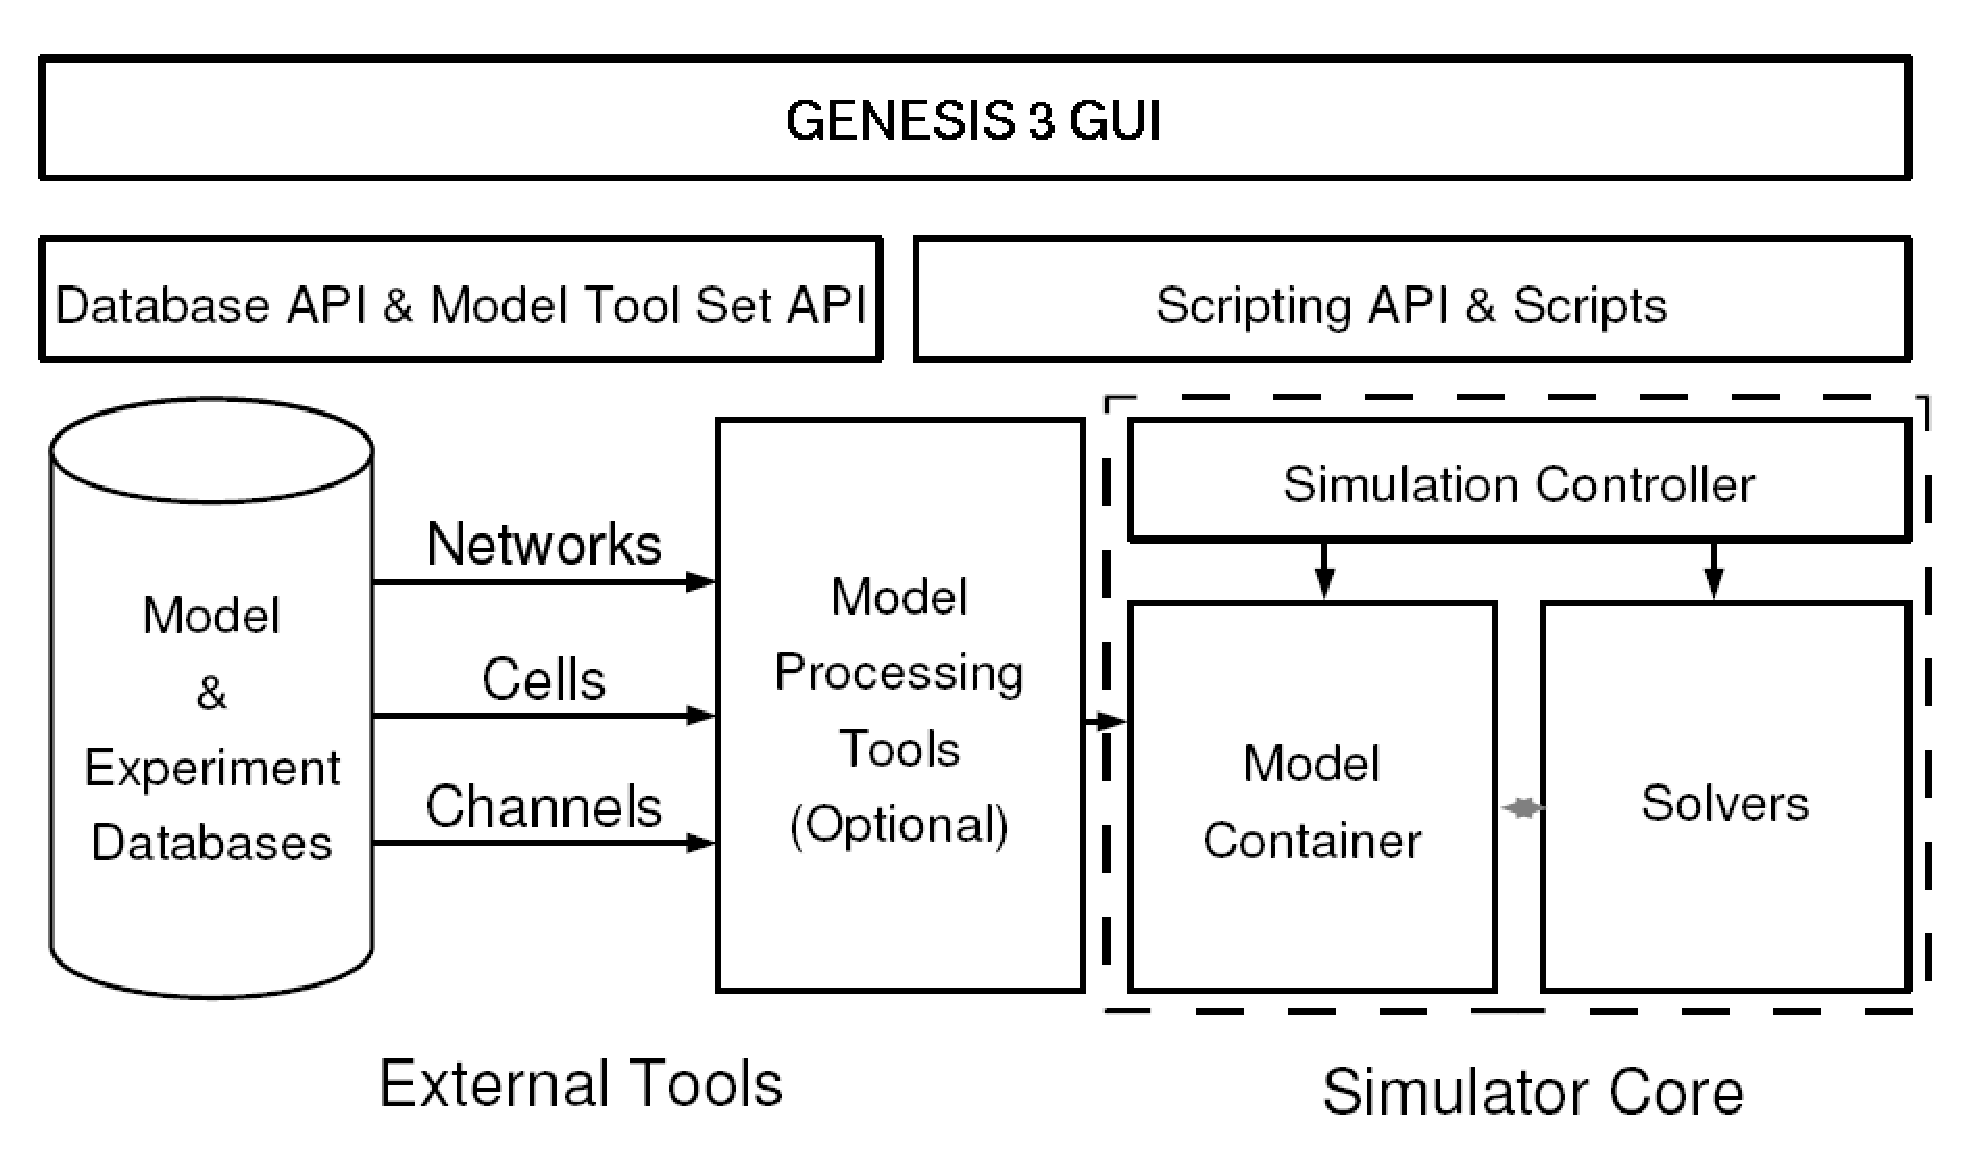
\includegraphics[scale=0.5]{figures/G3arch.eps}
\caption{
{\bf Relation of components in the Computational Biology Initiative (CBI) federated software architecture.} The CBI architecture defines the relationships between the necessary components of a computer-based neural simulation system. The architecture contains three layers that include a graphical user interface connected to the functional components of a simulator by an interposed layer of application programming interfaces. Components in the lowest layer are interconnected by application programming interfaces while their functionality is needed. GENESIS 3 is the first simulator to be implemented in compliance with the CBI architecture.
}
\label{fig:cbi-arch}
\end{figure}

\clearpage

%\section*{Tables}
%\begin{table}[!ht]
%\caption{
%\bf{Table title}}
%\begin{tabular}{|c|c|c|}
%table information
%\end{tabular}
%\begin{flushleft}Table caption
%\end{flushleft}
%\label{tab:label}
% \end{table}

\end{document}

